\section{Kinematics and Timing of Signal and Background events}


\subsection{0\nbb-decay signal and 2\nbb-decay background}

\begin{figure*}[ht]
  \centering
  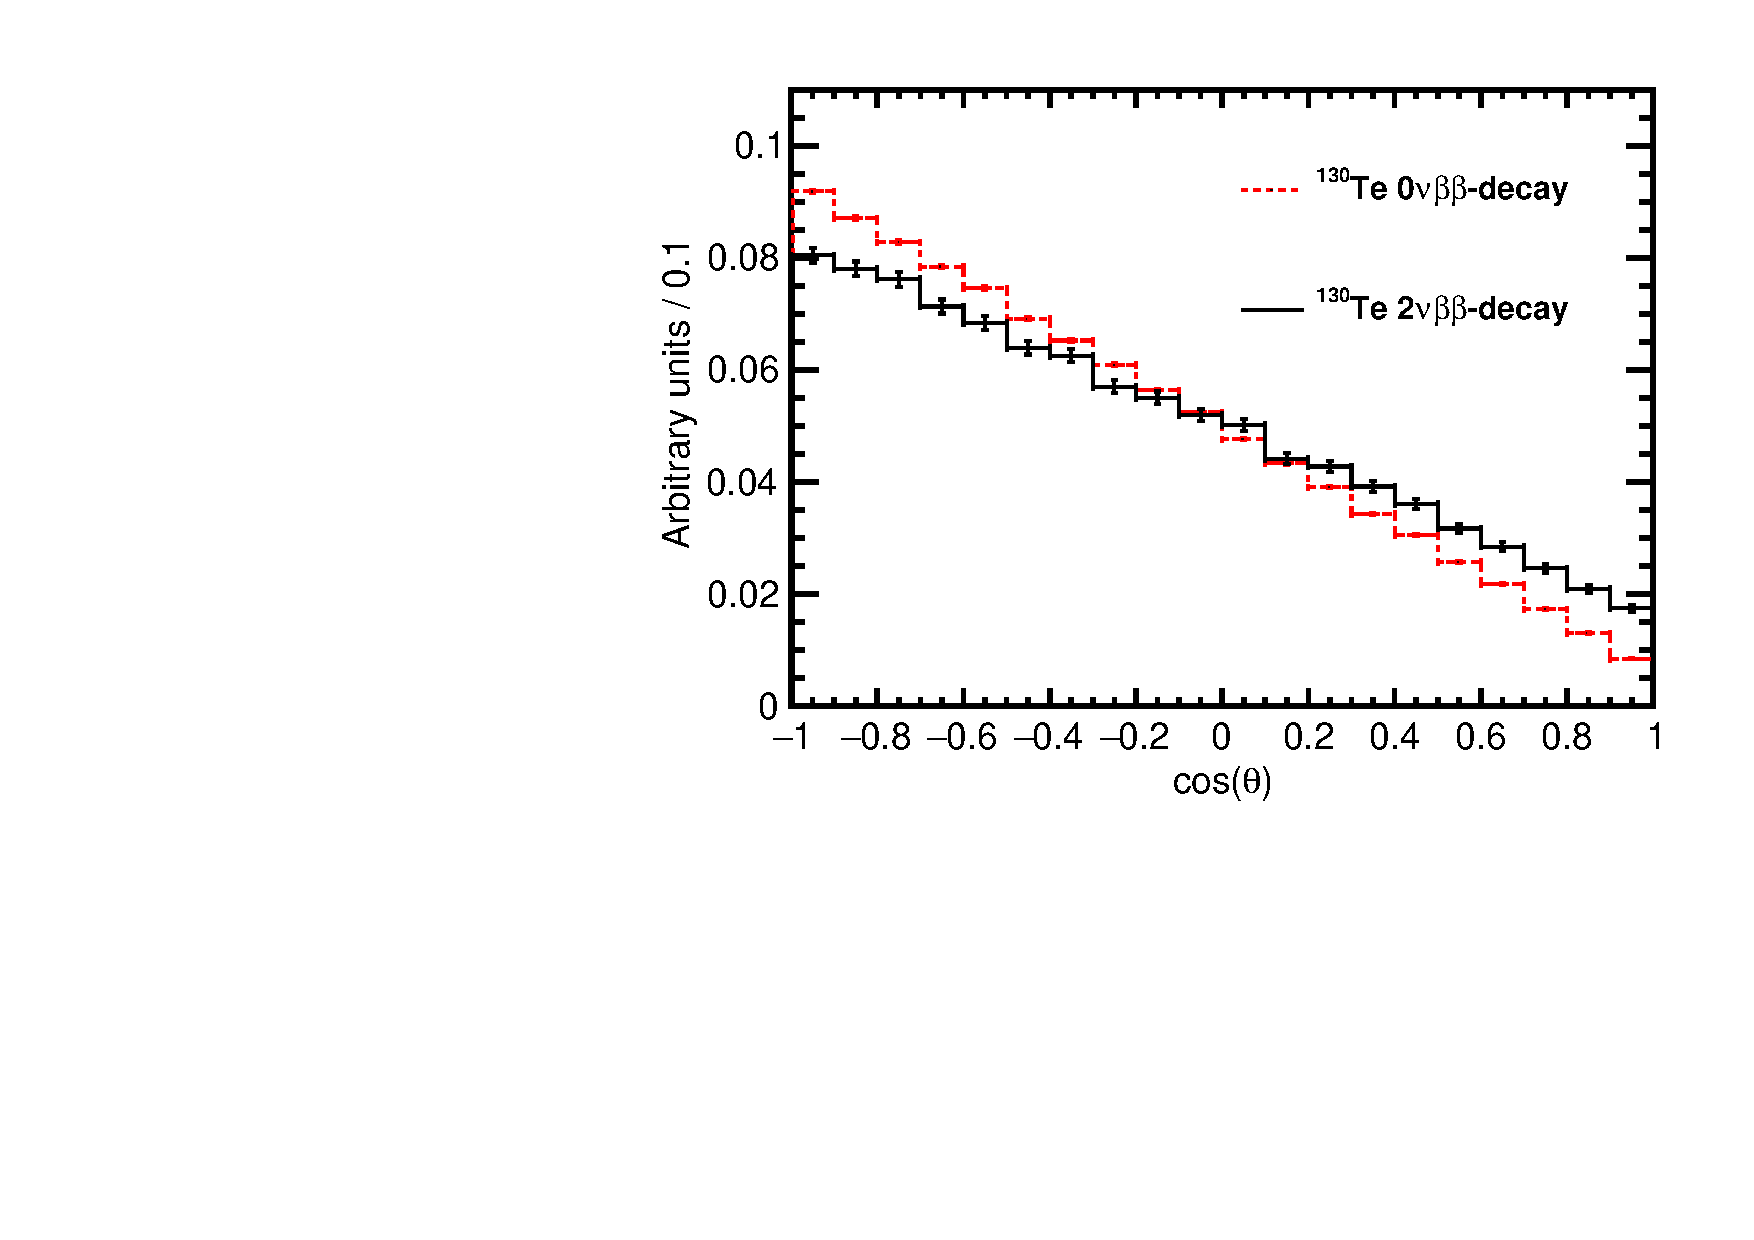
\includegraphics[width=0.49\textwidth]{hCos_Te130.pdf}
  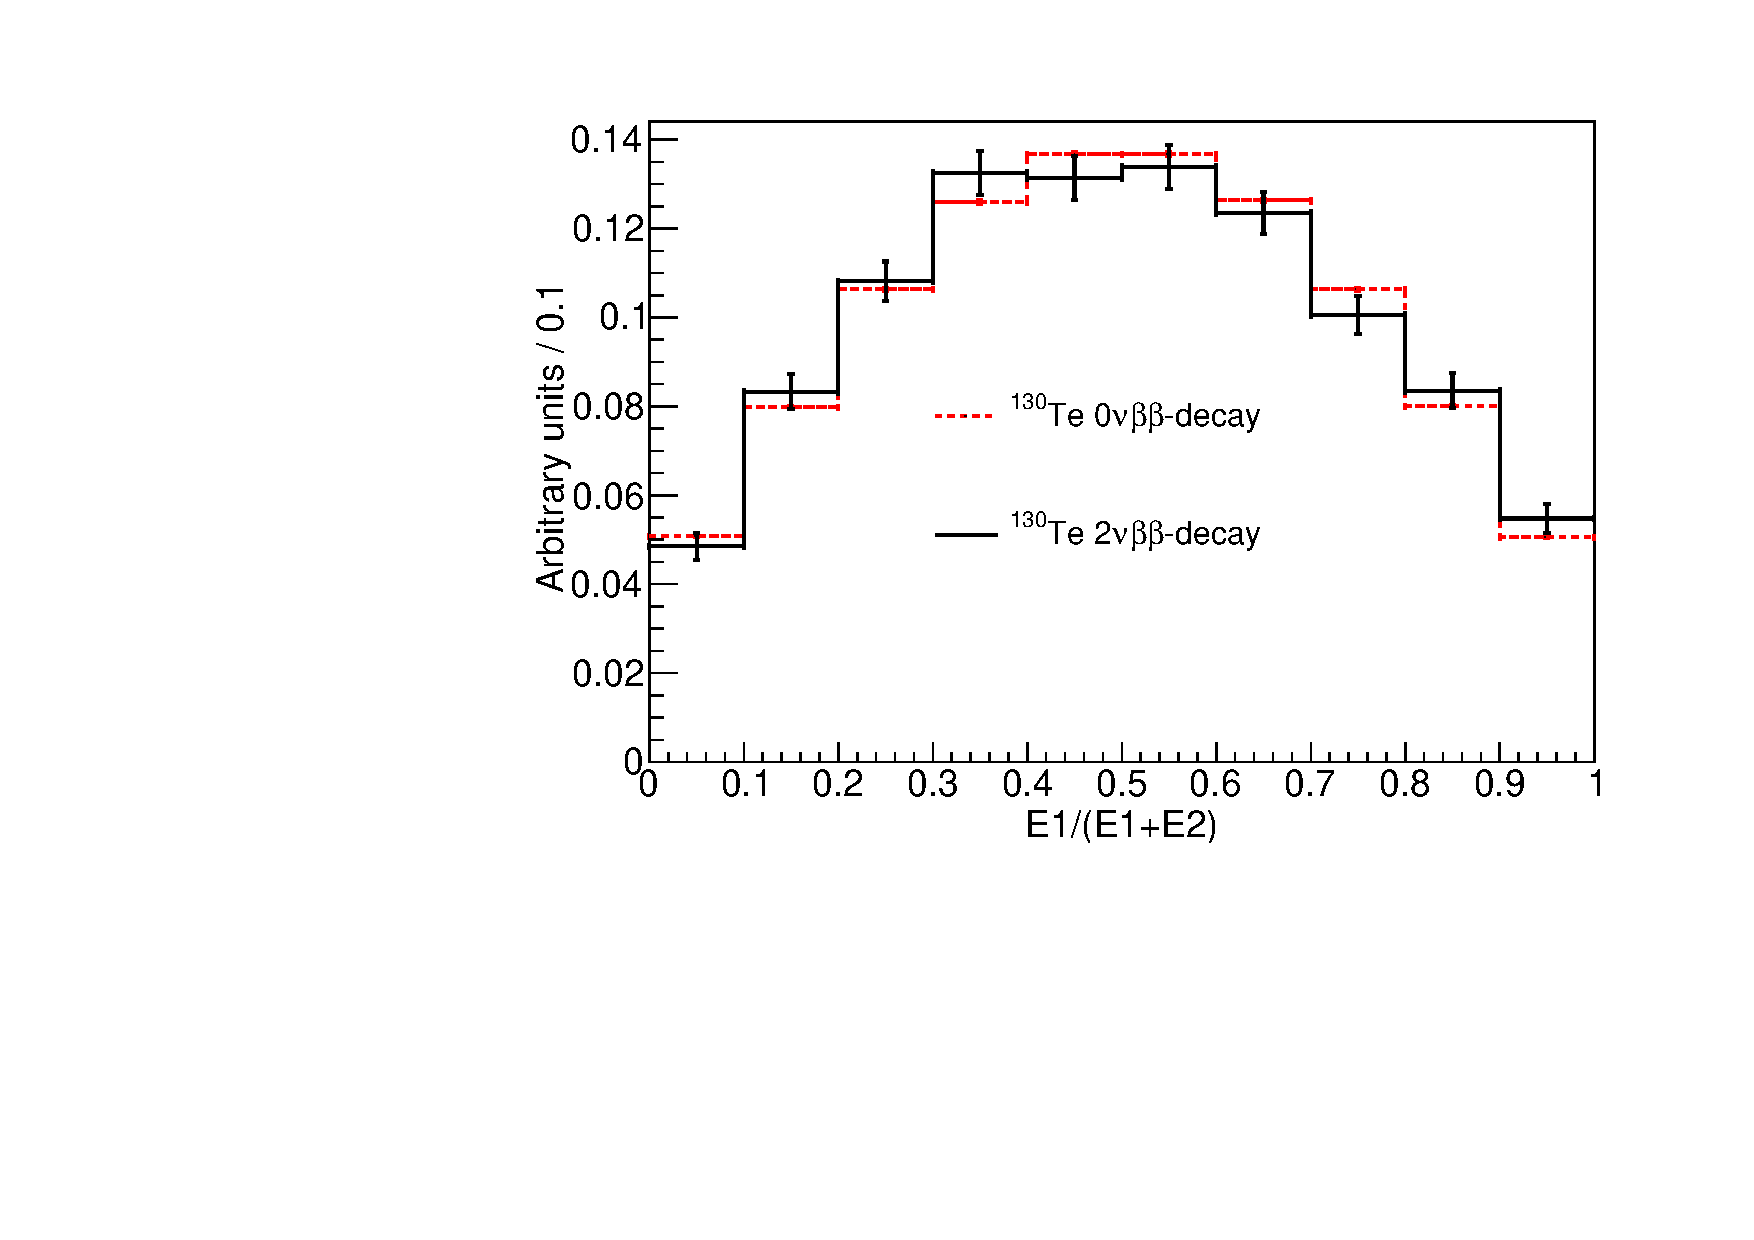
\includegraphics[width=0.49\textwidth]{hE1toQ_Te130.pdf}
  \caption{Comparison between kinematics of 0{\nbb} (\emph{dashed red
      lines}) and 2{\nbb} decays (\emph{solid black lines}) for events
    with the total kinetic energy of the electrons above 90\% of the
    Q-value. \emph{Left:} Cosine of the angle between two
    electrons. \emph{Right:} Fraction of energy carried by one of the
    two electrons. Due to limited statistic around the energy spectrum
    end point for 2{\nbb} decay we show statistical errors for each
    bin.}
  \label{fig:Kinematics}
\end{figure*}


\begin{figure*}[ht]
  \centering
  %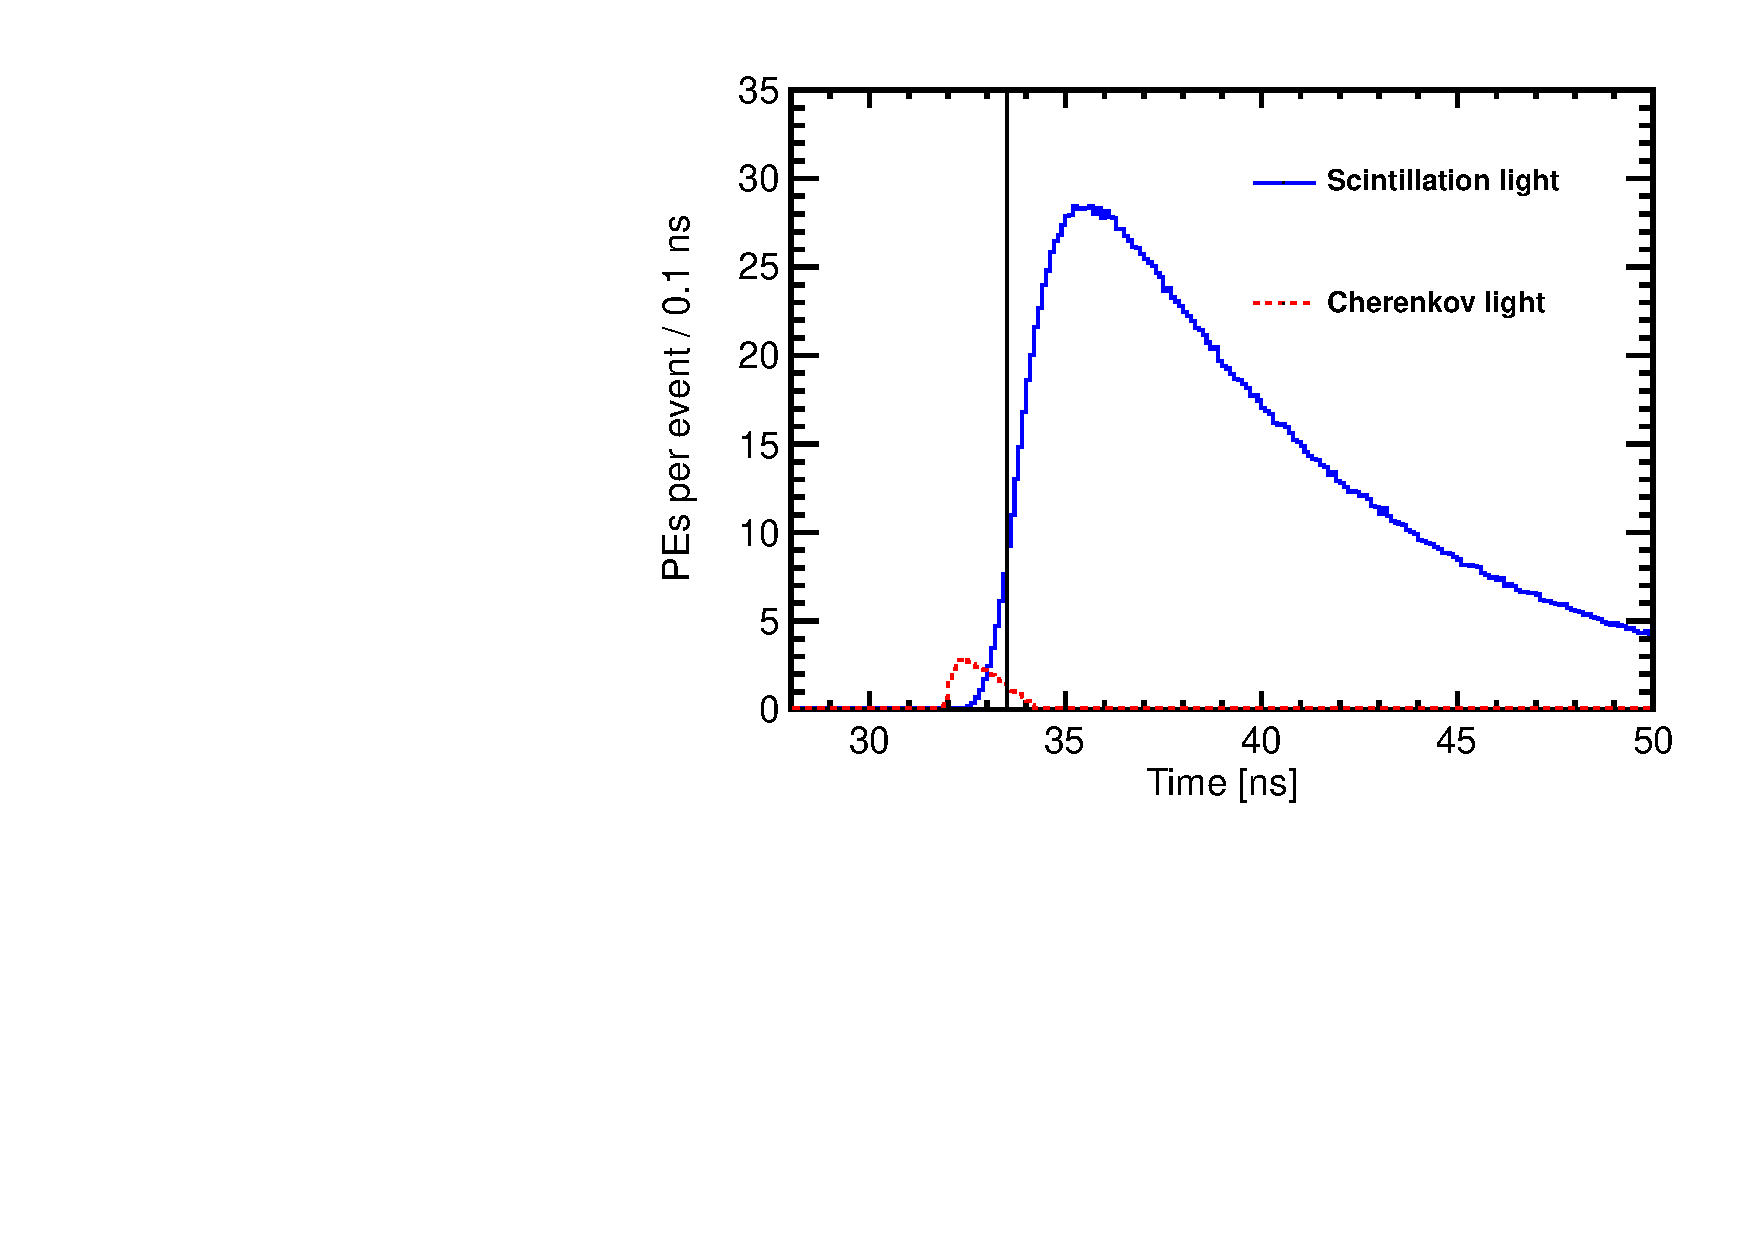
\includegraphics[width=0.45\textwidth]{hT_Te130.pdf}
  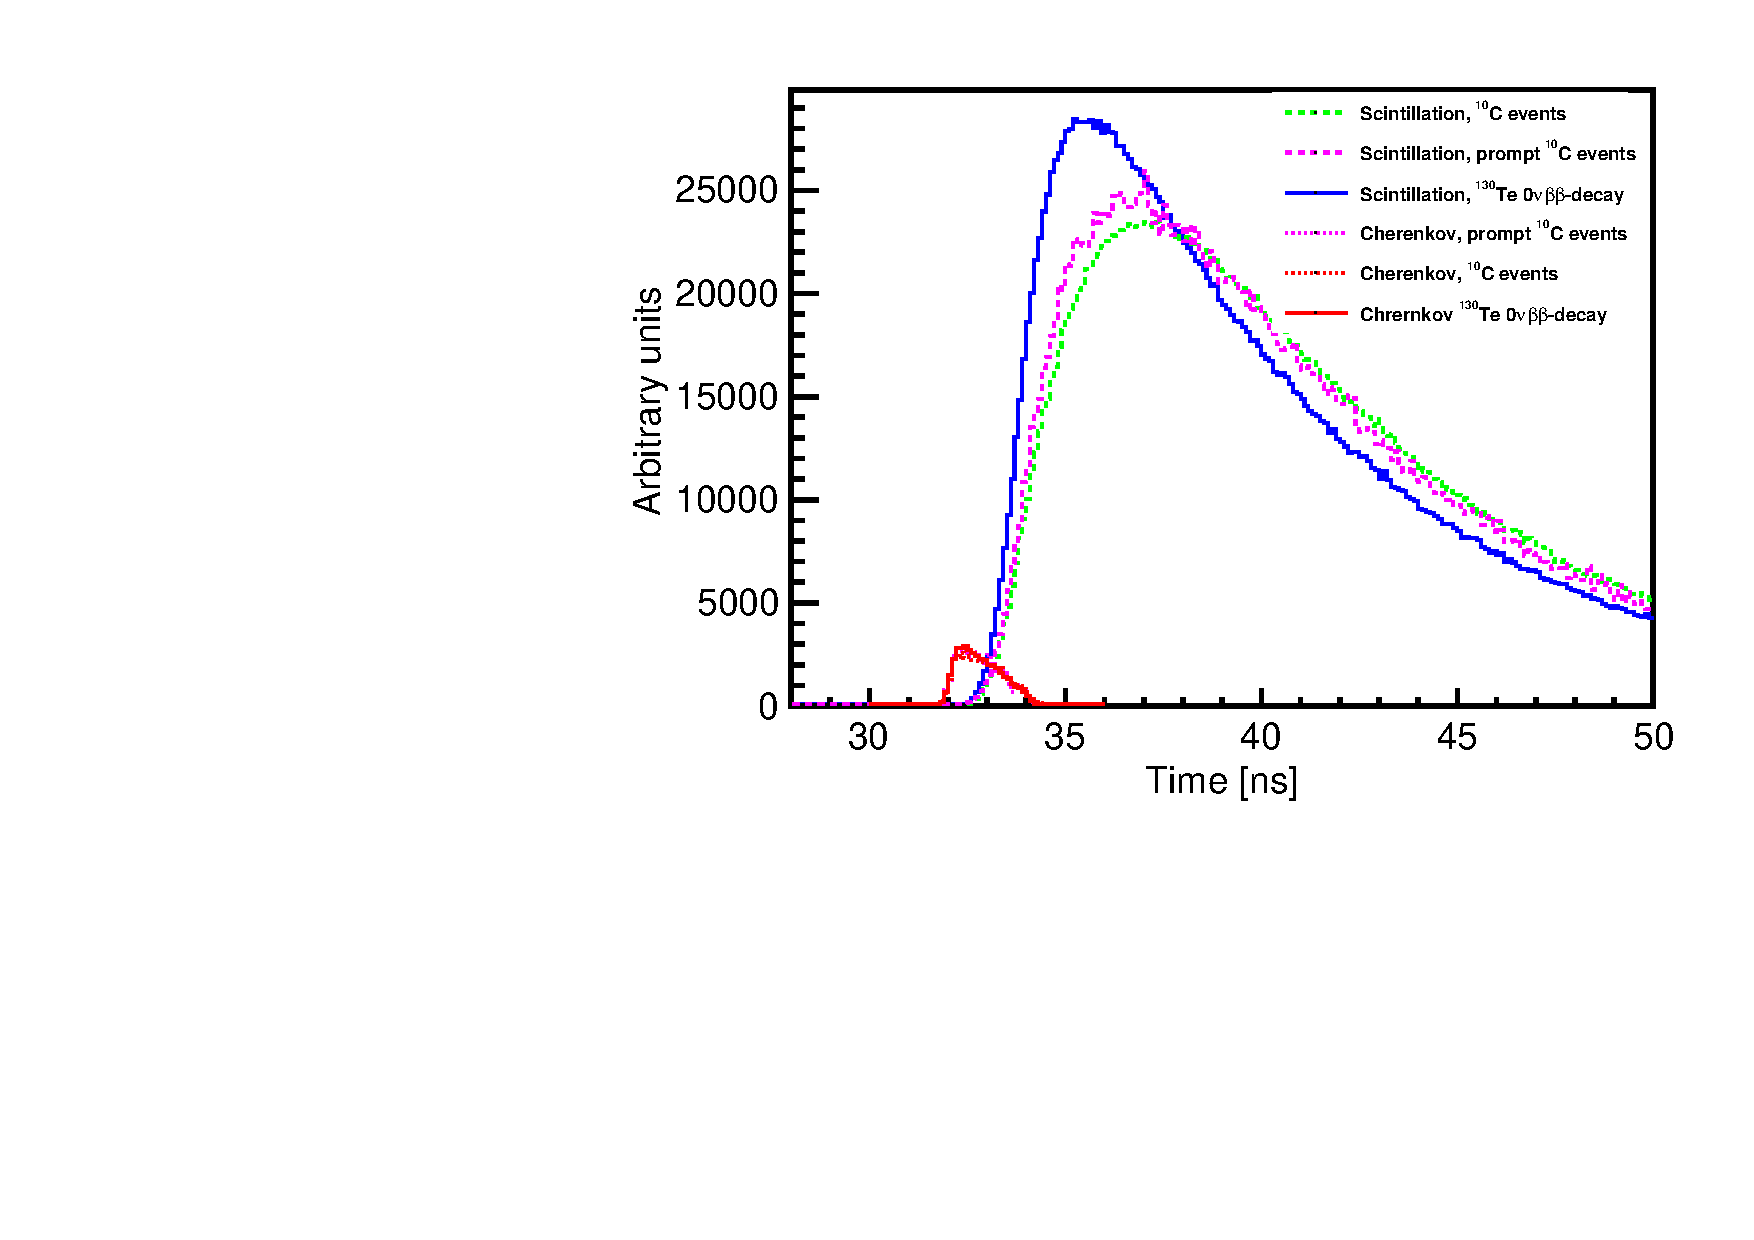
\includegraphics[width=0.45\textwidth]{hT_Te130vsC10_overlaid_v2.pdf}
  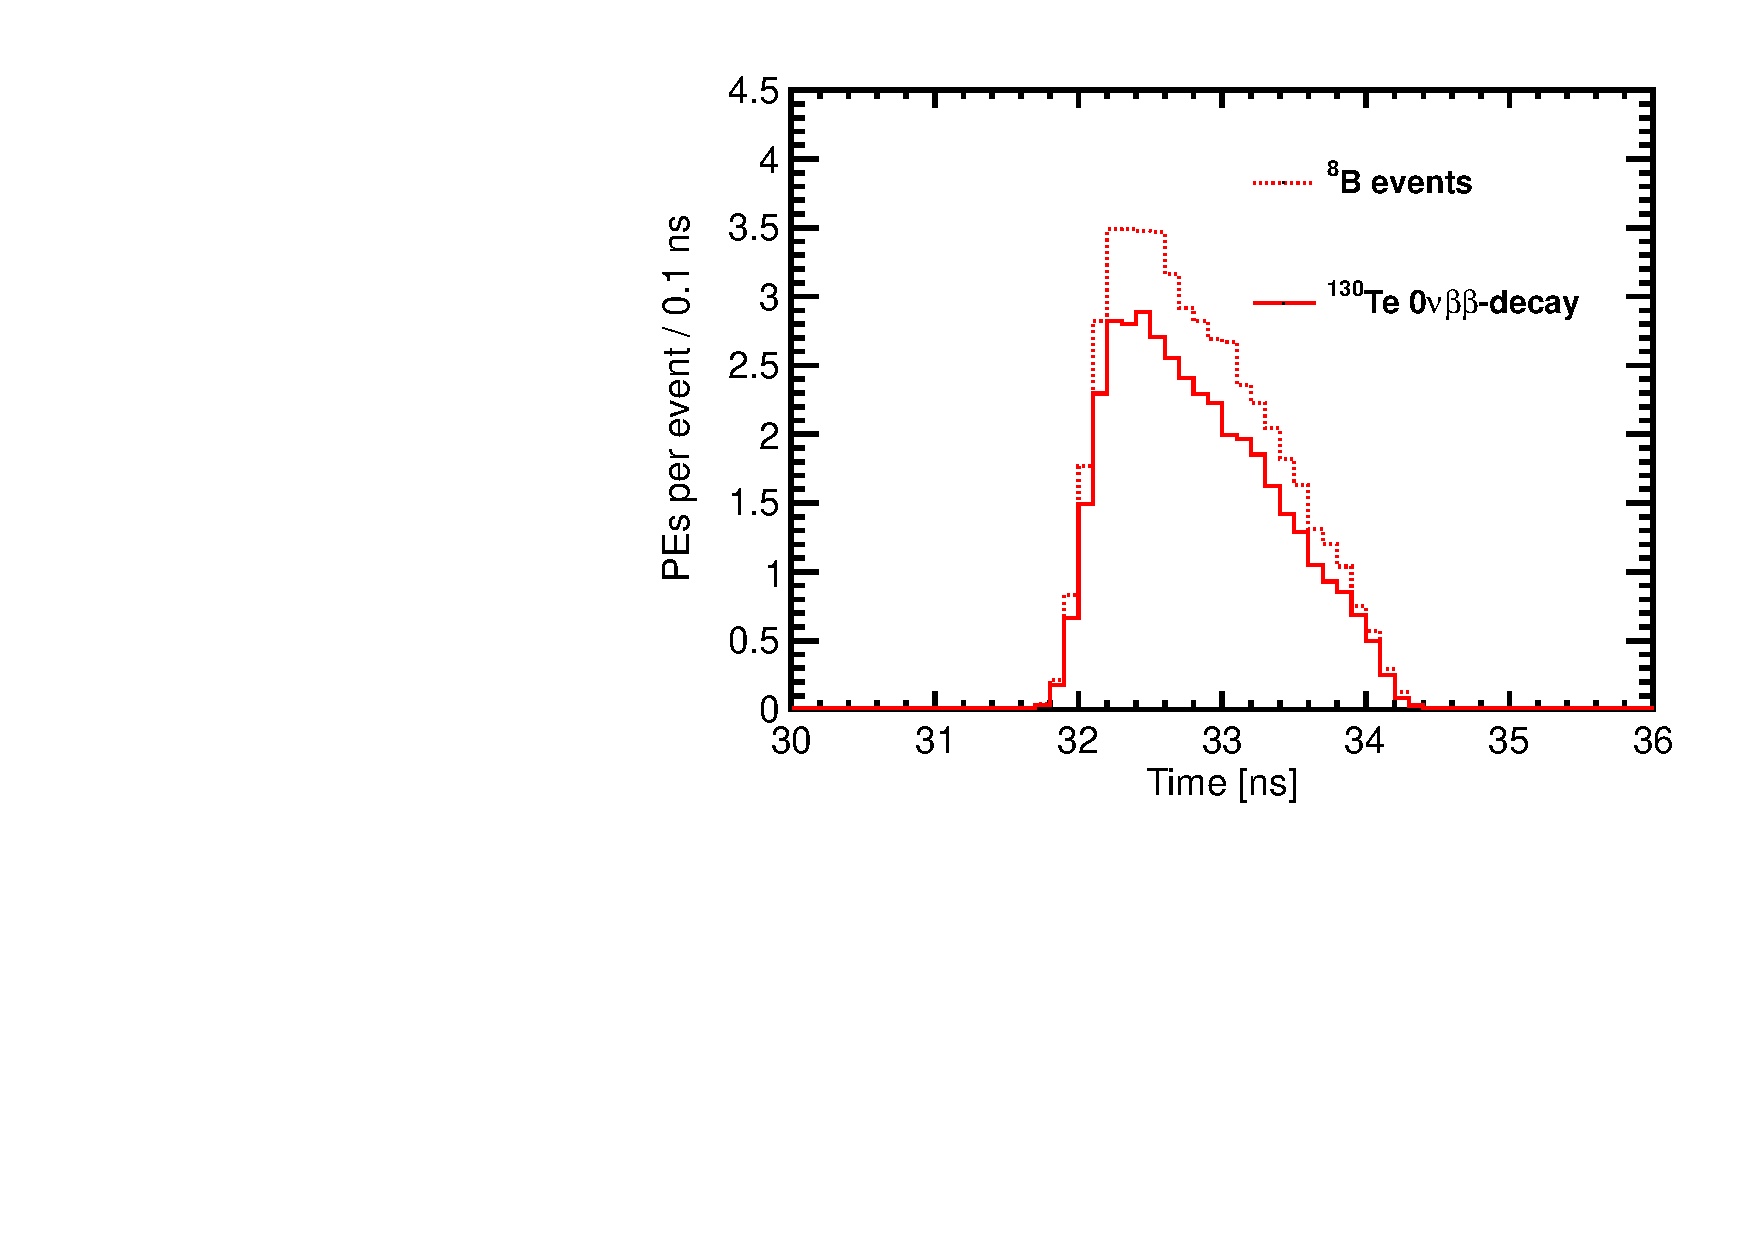
\includegraphics[width=0.45\textwidth]{hTche_Te130_B8.pdf}
  \caption{\emph{Left:} Photo-electron (PE) arrival times after
    application of the photo-detector transit time spread (TTS) of
    100~ps for the simulation of 1000 0{\nbb} decay events of
    $^{130}$Te at the center of the detector. PEs from Cherenkov light
    (\emph{dashed red line}) and scintillation light (\emph{solid blue
      line}) are compared. The black vertical line illustrates a time
    cut at 33.5 ns. \emph{Right:} Comparison between Cherenkov PEs
    arrival time for $^{130}$Te {0\nbb} decay (\emph{solid line}) and
    $^{8}$B (\emph{dotted line}) events. {\bf Distributions of the
      scintillation PEs arrival time are indistinguishable between
      $^{130}$Te 0{\nbb} decay and $^8$B due to identical total energy
      in the event, $Q(^{130}{\rm Te})=2.526$~MeV.} }
\label{fig:ArrivalTimeDist}
\end{figure*}


\begin{figure*}[ht]
  \centering
  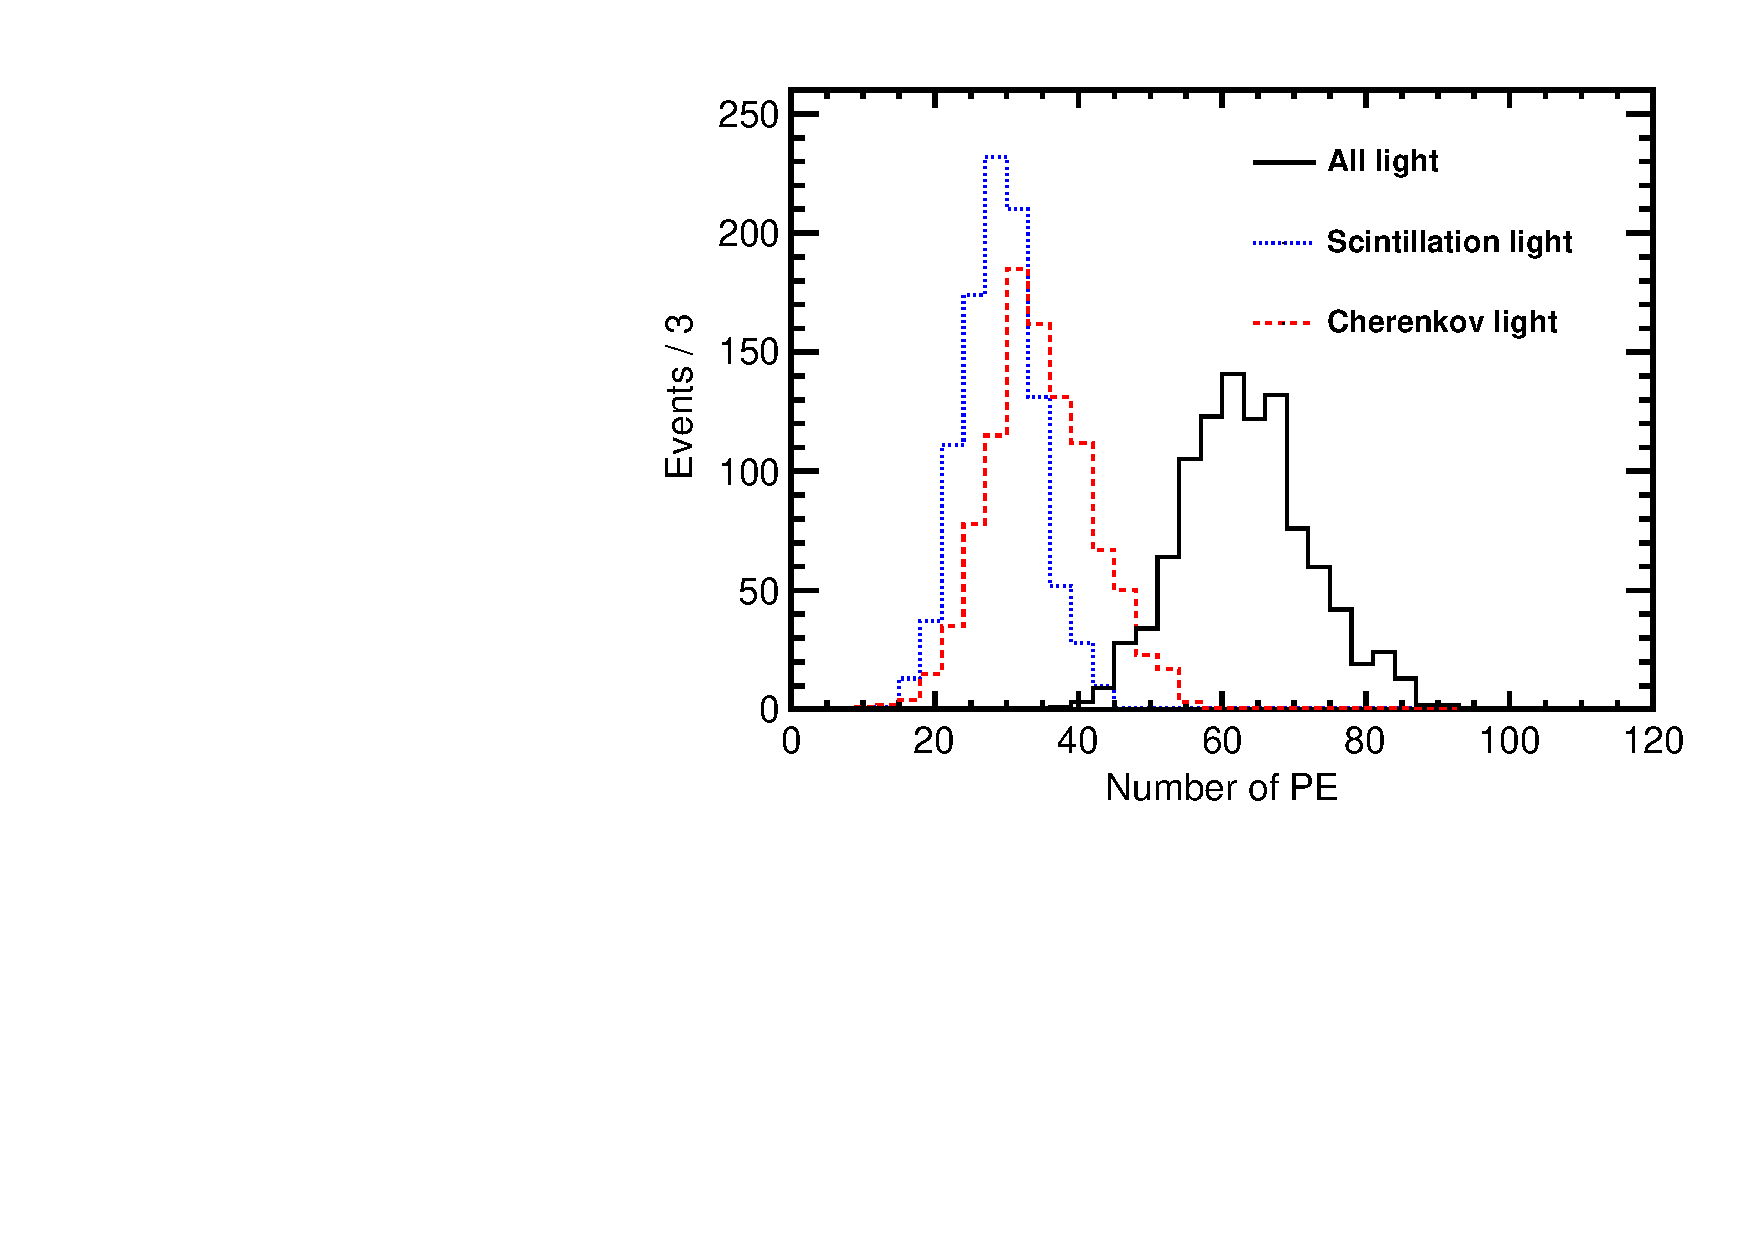
\includegraphics[width=0.33\textwidth]{hMomNPhot_Te130.pdf}
  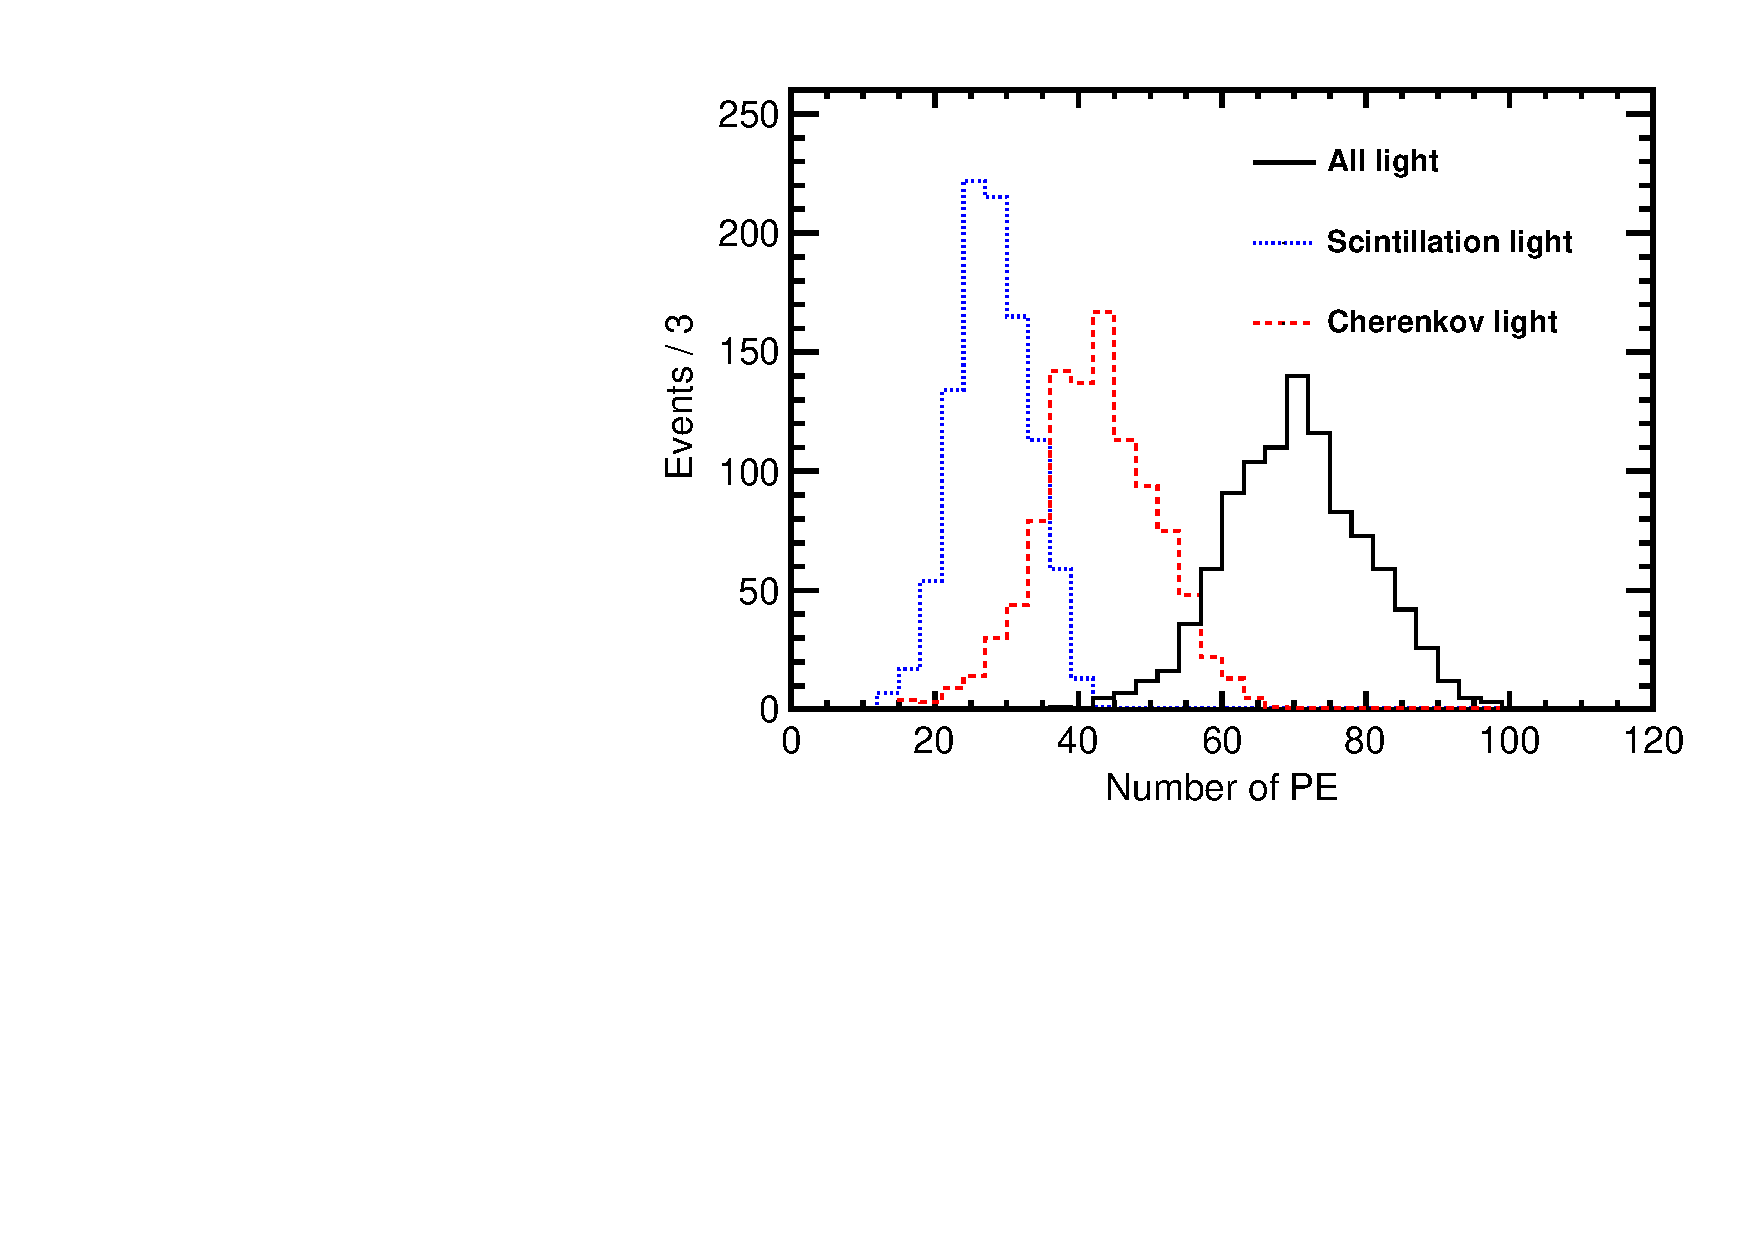
\includegraphics[width=0.33\textwidth]{hMomNPhot_1el_2p529MeV.pdf}
  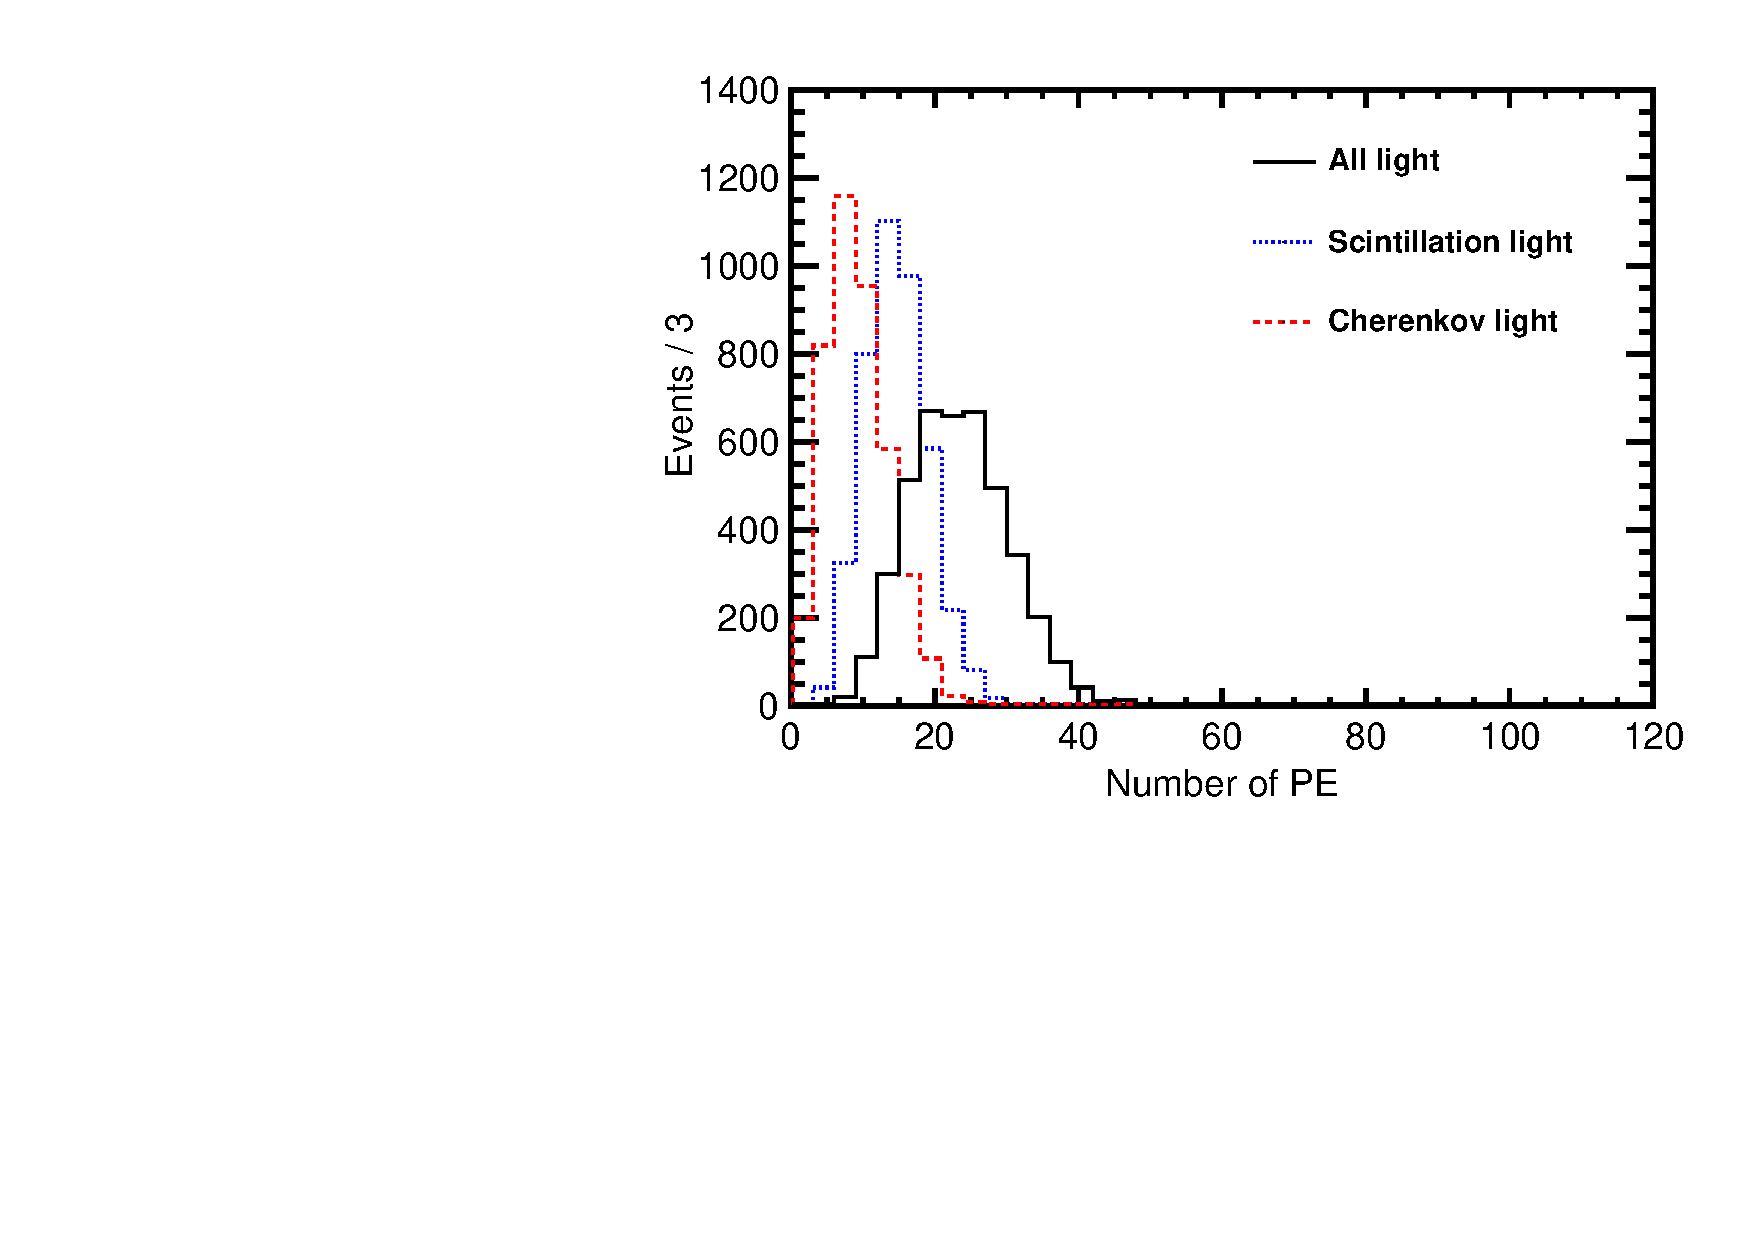
\includegraphics[width=0.33\textwidth]{hMomNPhot_C10.pdf}
  \caption{Number of Cherenkov (\emph{dashed red line}), scintillation
    (\emph{dotted blue line}), and total (\emph{solid black line}) PEs
    for the simulation of 1000 $^{130}$Te 0{\nbb} decay (left panel)
    and $^8$B (\emph{right panel}) events.}
\label{fig:NPhotDist}
\end{figure*}






\subsection{\B~background}



\subsection{\C~background}


\begin{figure}[ht]
  \centering
  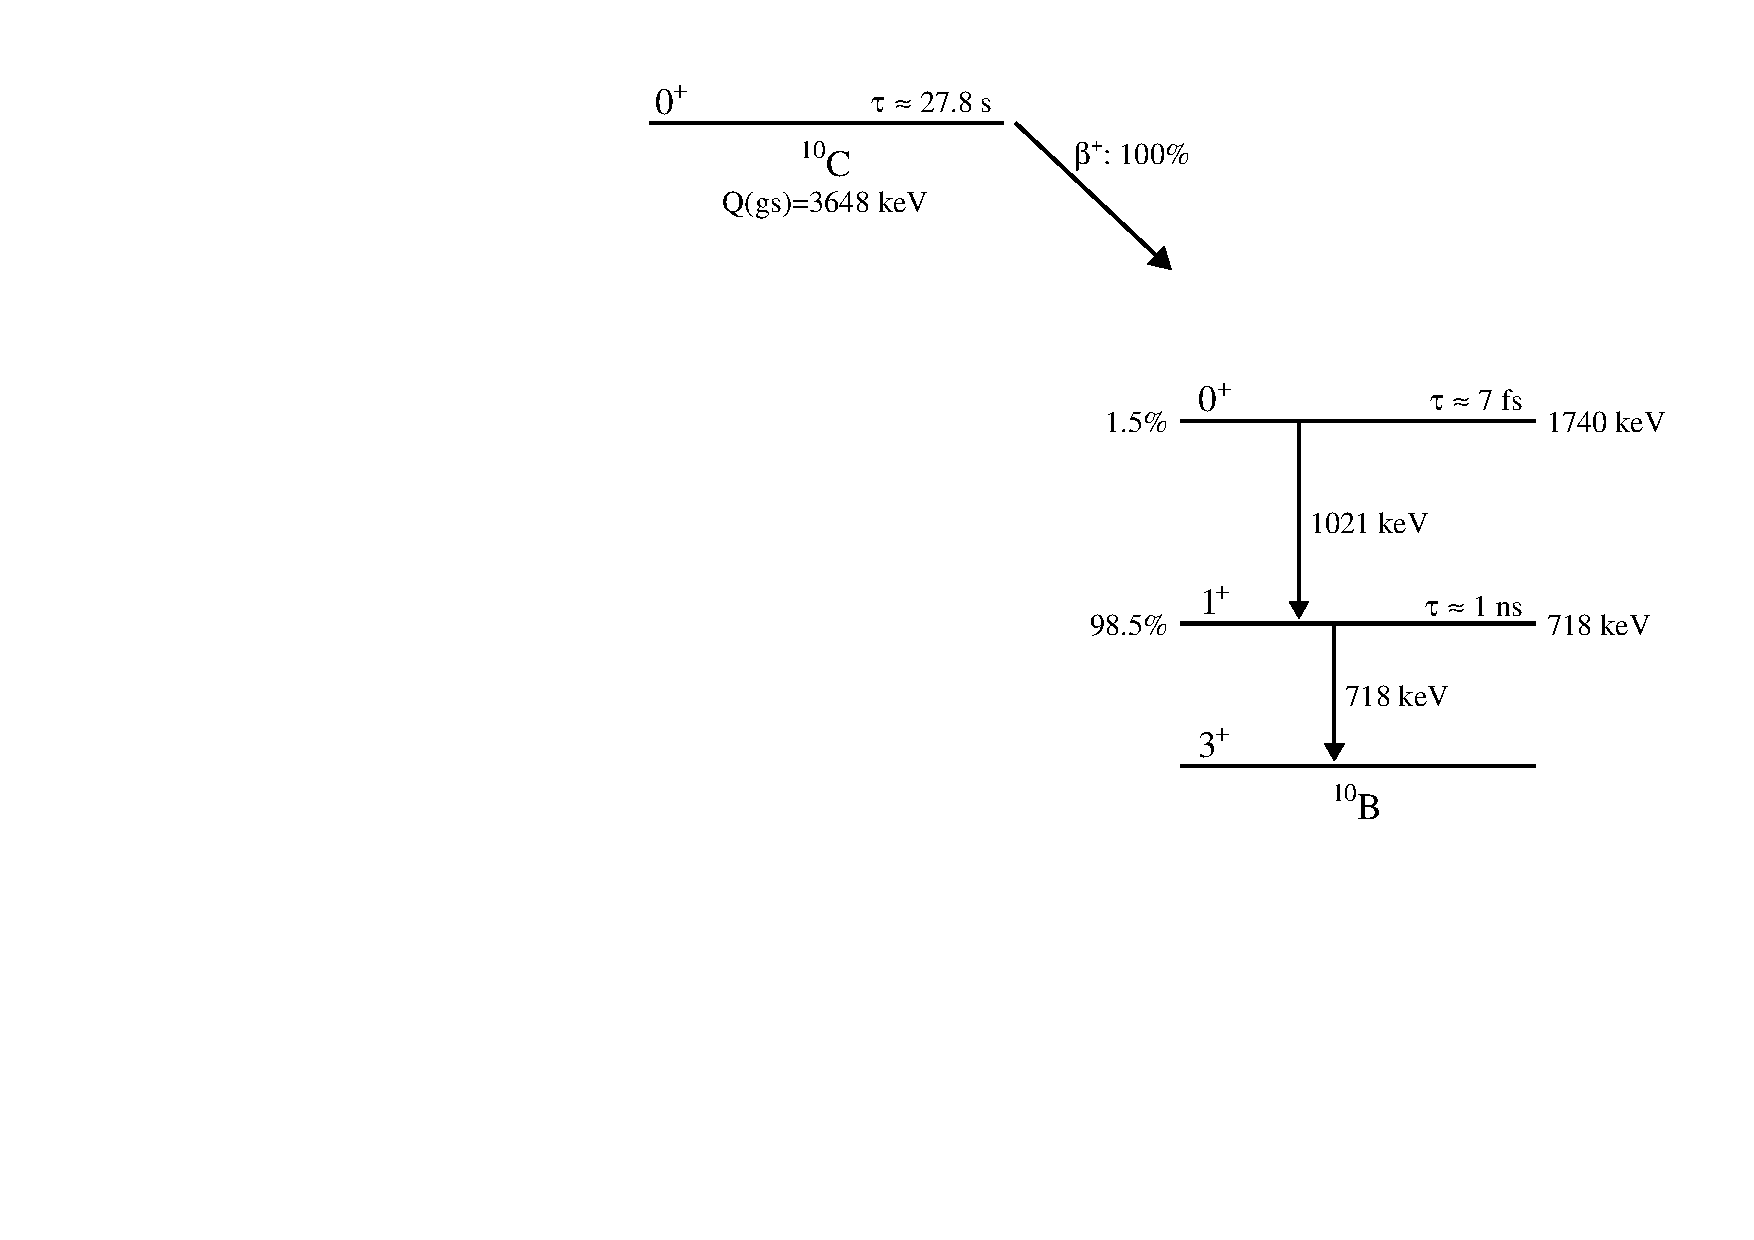
\includegraphics[width=0.49\columnwidth]{C10DecayScheme.pdf}
  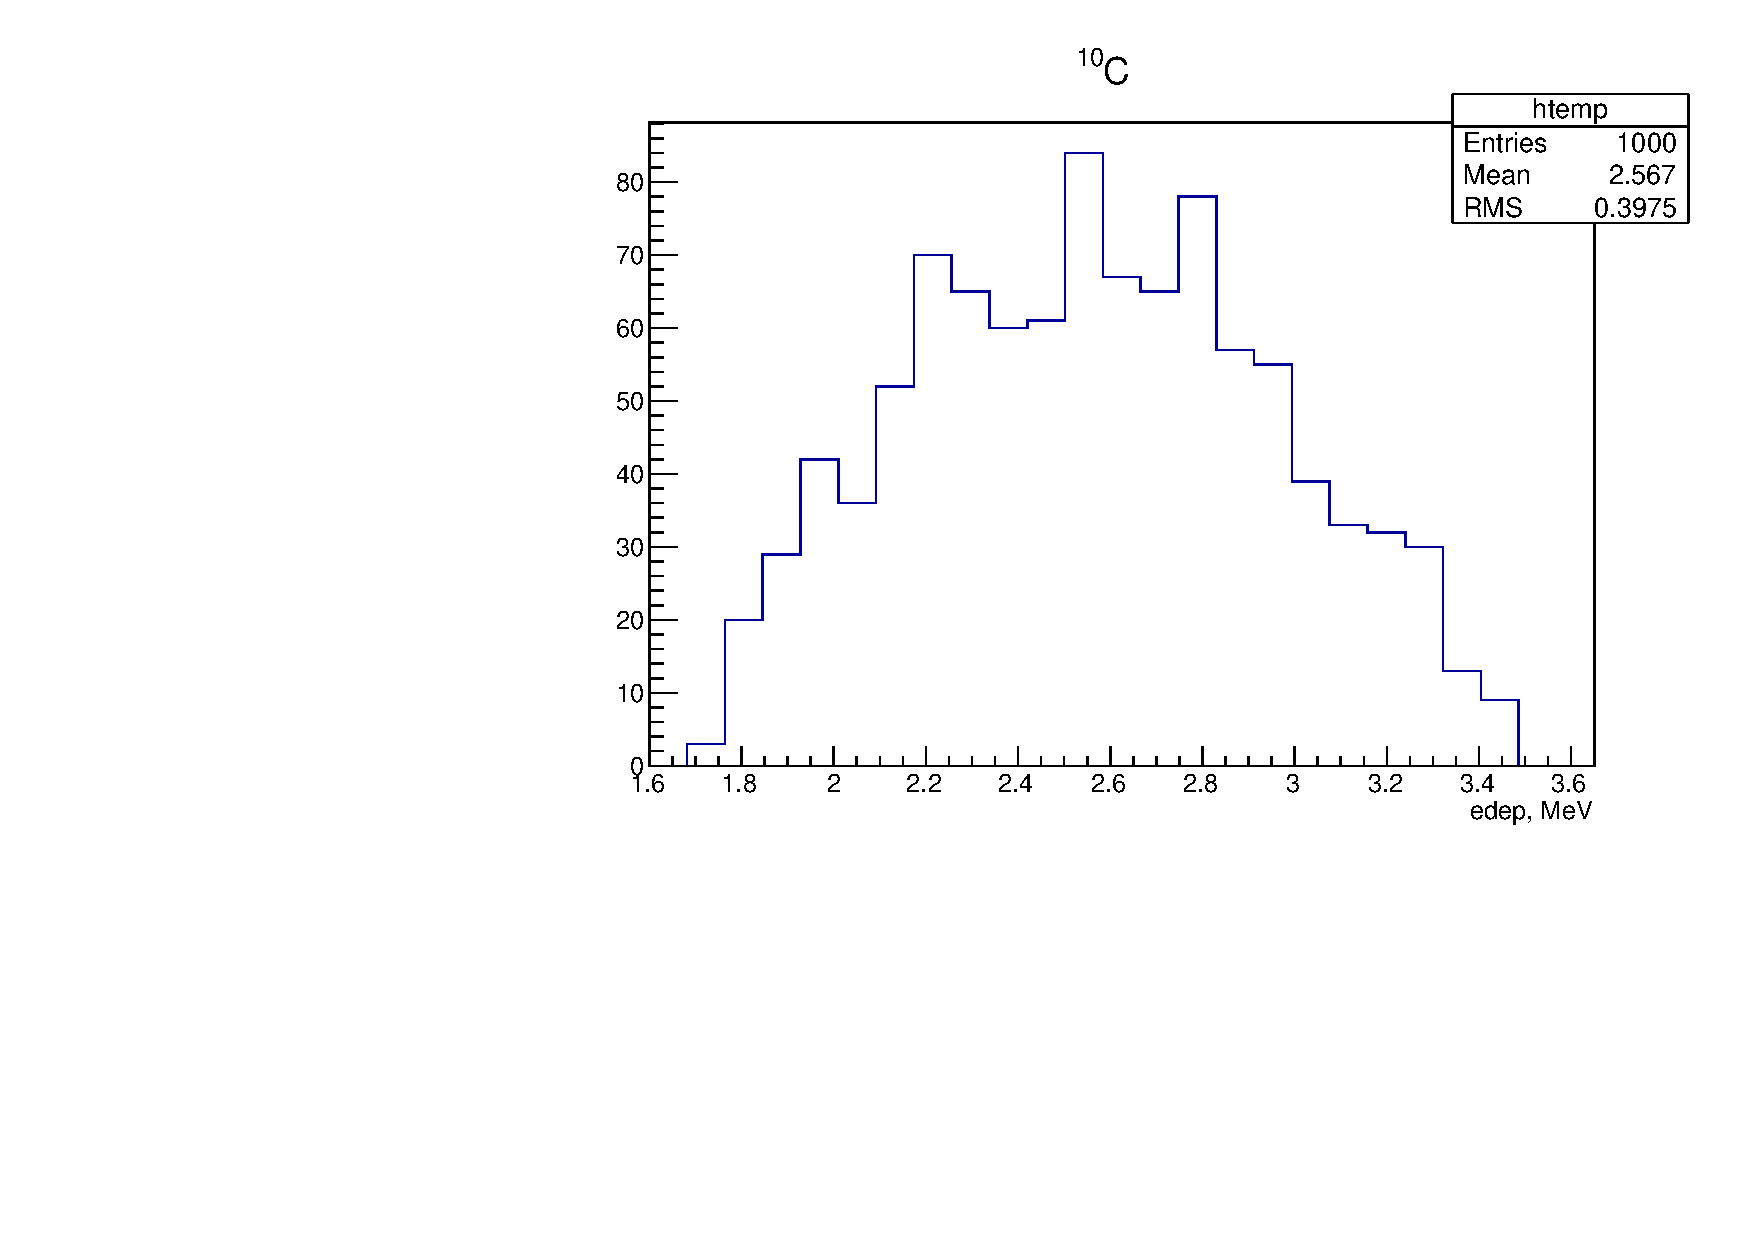
\includegraphics[width=0.49\textwidth]{hEdep_C10.pdf}
  \caption{\emph{Left:} Decay scheme of \C~events. \emph{Rigth:} Energy deposition in \C~events. Vertical solid line indicates 2.53~MeV
    which corresponds to Q-value of \Te~isotope. Vertical dashed lines indicate 2.28~MeV and 2.78~MeV which correspond to $\pm$10\% region 
    around the Q-value.}
\label{fig:C10_scheme_and_edep}
\end{figure}




\subsection{0\nbb/\C~separation using PE timing}
\begin{figure}[h]
  \centering
  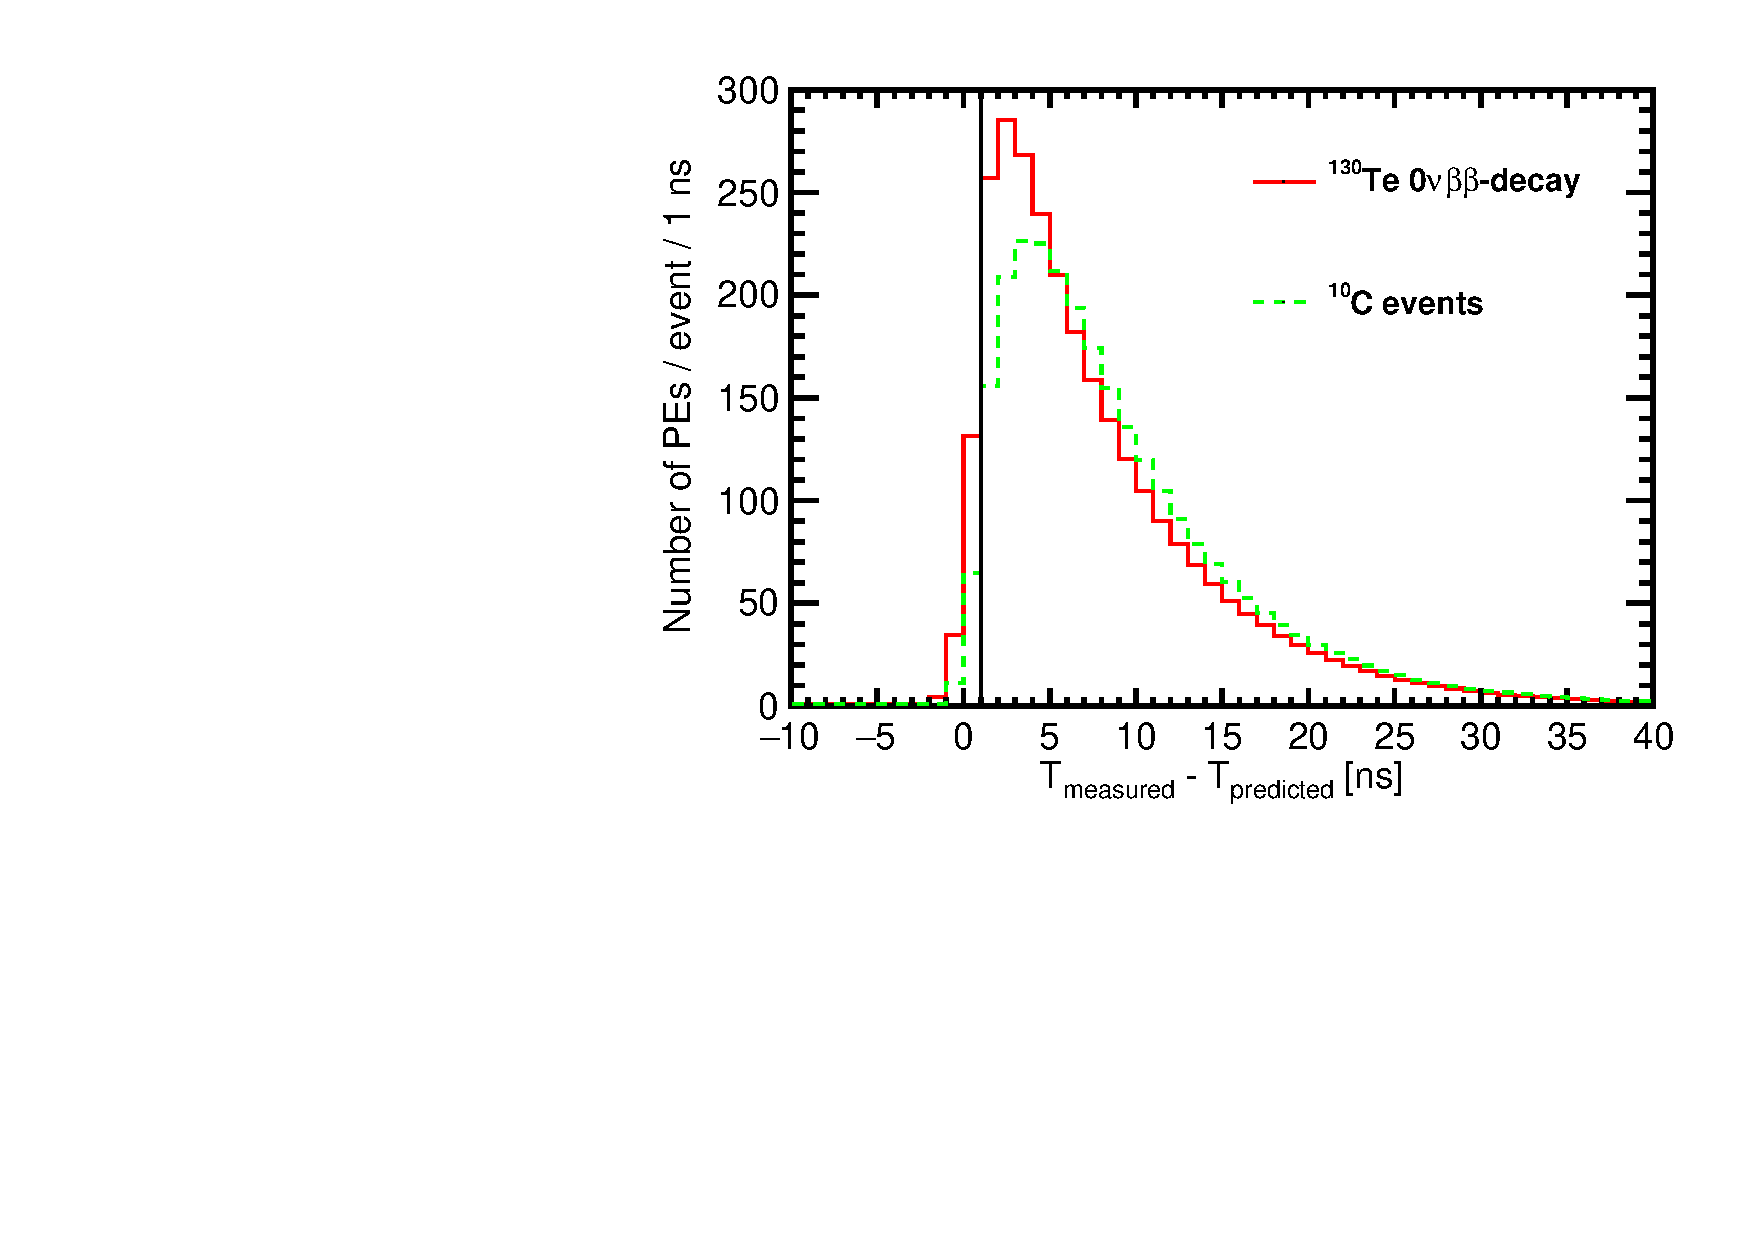
\includegraphics[width=0.45\textwidth]{hMomDT_Te130vsC10_allLight_VtxSmear3cm_VtxShiftX0cm_momDT1p0ns_rndVtx_3p0mSphere.pdf}
  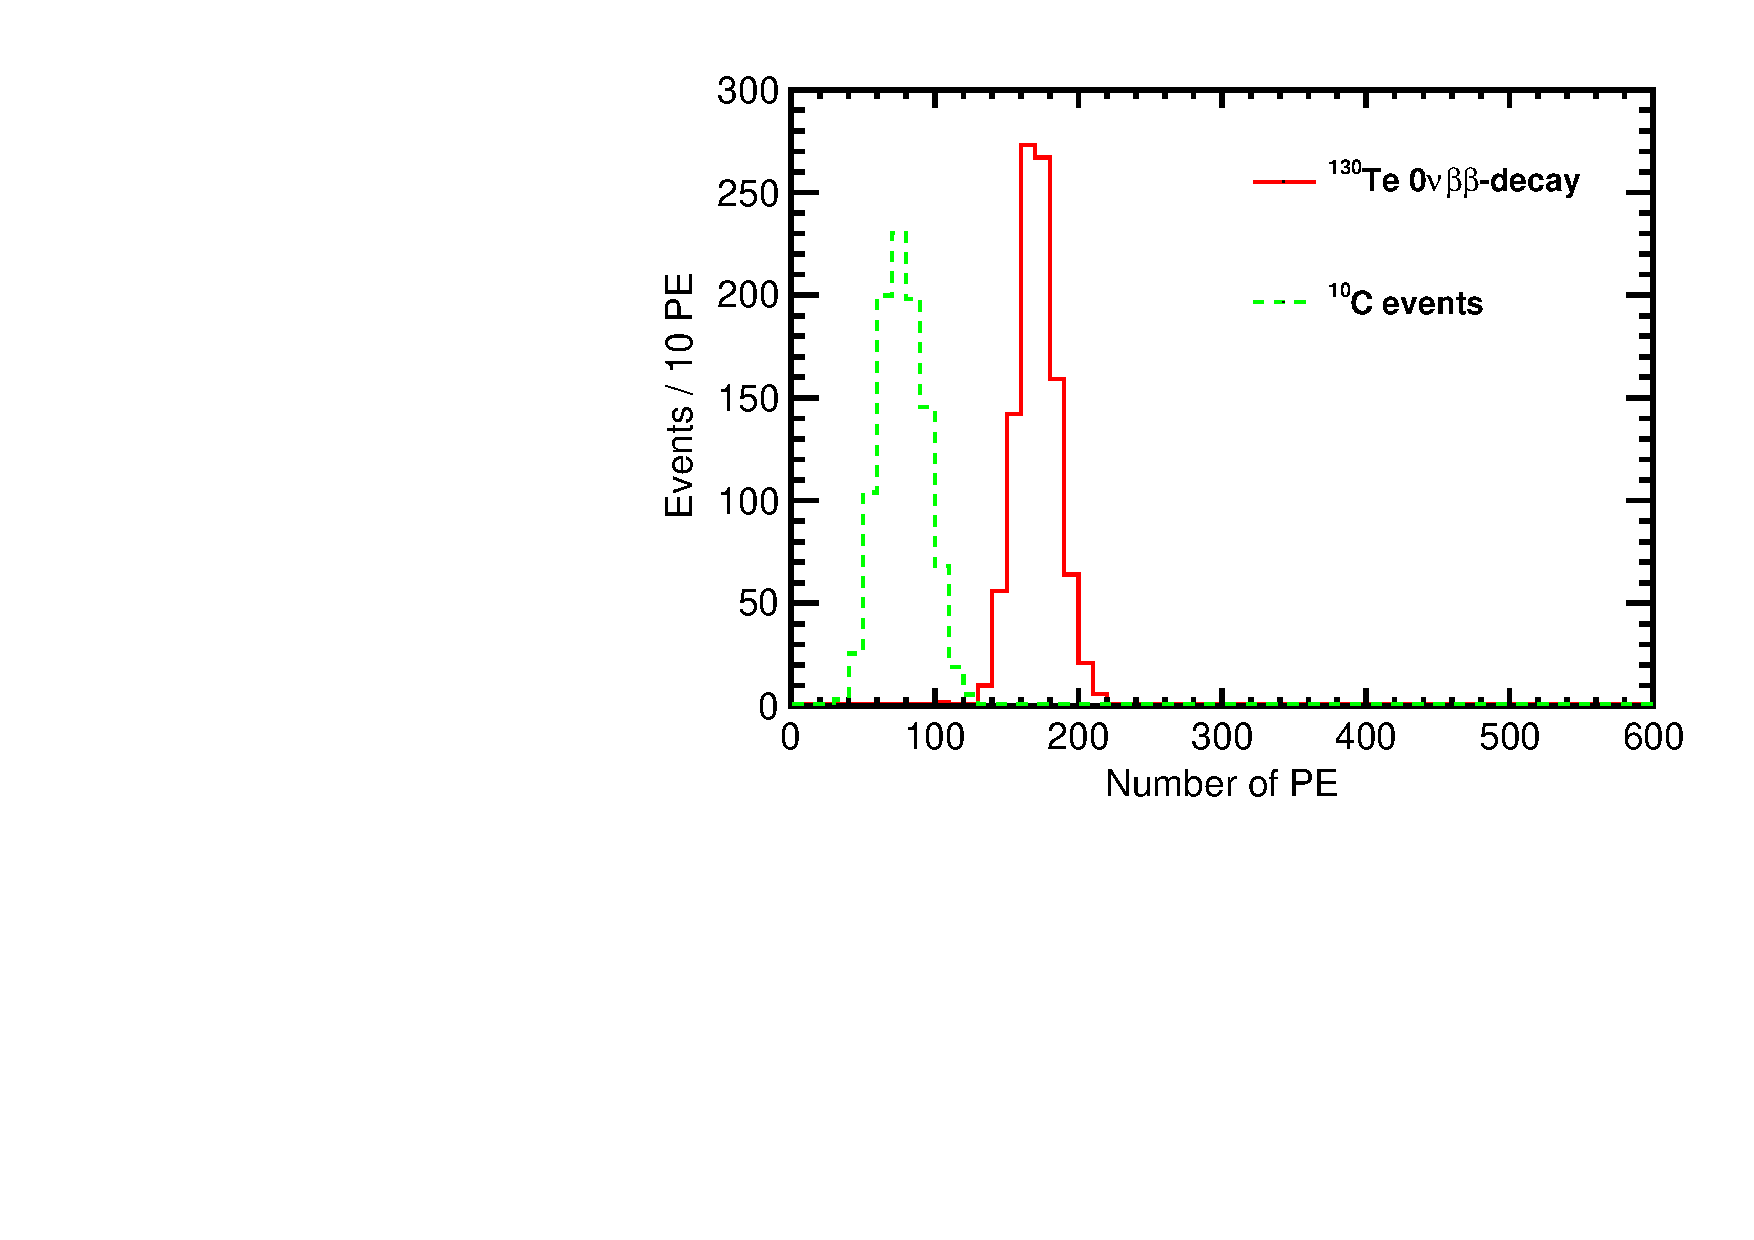
\includegraphics[width=0.45\textwidth]{hMomNPhot_Te130vsC10_allLight_VtxSmear3cm_VtxShiftX0cm_momDT1p0ns_rndVtx_3p0mSphere.pdf}
  \caption{}
\label{fig:0nbb-C10_timing_separation}
\end{figure}

